\newprob{1718611241}
{
    % Active physics p179 q4
    某枚  \qty{100}{\ohm} 的電阻器接駁至正弦交流電源。流經 該電阻器的電流,頻率為 \qty{20}{Hz},峯值為 \qty{3}{A}。
    \begin{parts}
        \part 求電阻器所消耗的平均功率。\zzh{2}
        \part 若電流的頻率上升,則平均功率有何變化? 增大、減小還是保持不變?\zzh{1}
    \end{parts}
}{
    % \src{Active physics p179 q4}
    \par{\par\centering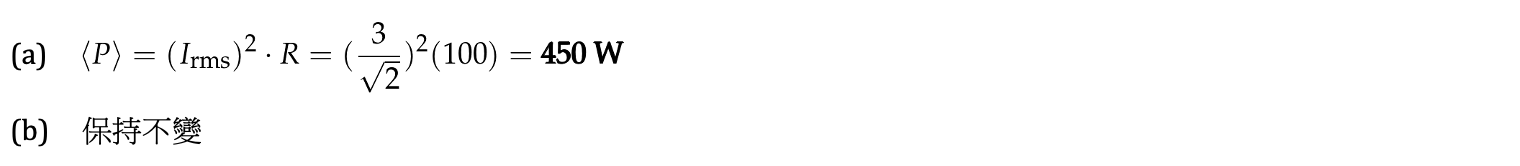
\includegraphics[width=\textwidth]{./img/ch_ACtransformer_lq_2024-06-17-20-34-20.png}\par}
}

\newprob{1718625571}
{
    % Active physics p179 q5
    一道穩定的 10 A 直流電通過某電阻器,十秒內 消耗電能 $E$。若改以另一正弦交流電向電阻器供 電,則同等時間內電阻器所消耗的電能為 $6E$。 求該交流電流的峯值。\zzh{2}
}{
    % \src{Active physics p179 q5}
    \par{\par\centering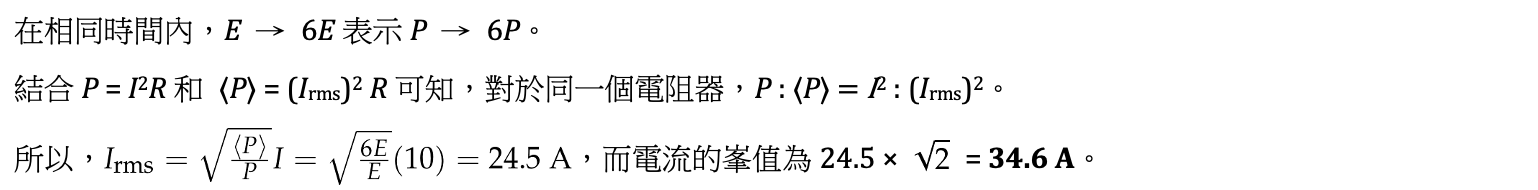
\includegraphics[width=\textwidth]{./img/ch_ACtransformer_lq_2024-06-17-20-34-42.png}\par}
}

\newprob{1718625635}
{
    % Active physics p179 q12
    以兩個不同的電源先後向相同的電阻器供電,流 經電阻器的電流如圖隨時間$t$變化。注意 (b)部 圖中的曲線部分是正弦曲線。
    \par{\par\centering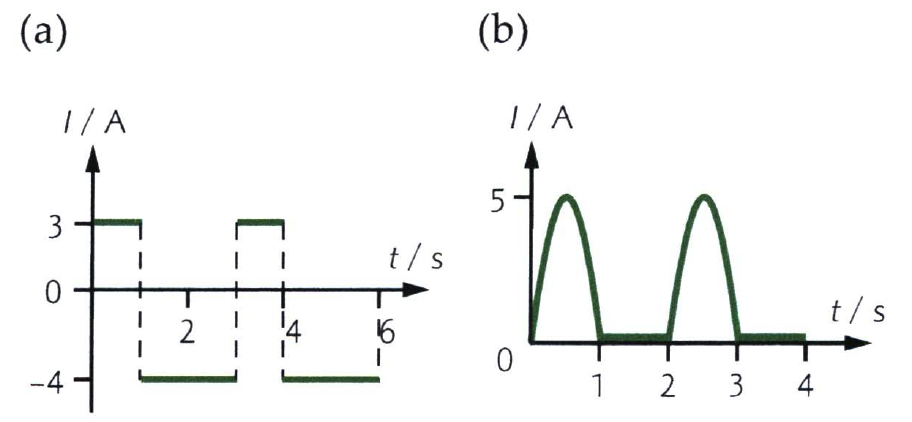
\includegraphics[width=.5\textwidth]{./img/ch_ACtransformer_lq_2024-06-17-20-01-07.png}\par}
    考慮一週期中所消耗的能量,若有一穩定直流電 可提供同等的熱效應,問此直流電之電流為多 少?\par\zzh{4}
}{
    % \src{Active physics p179 q12}
    \par{\par\centering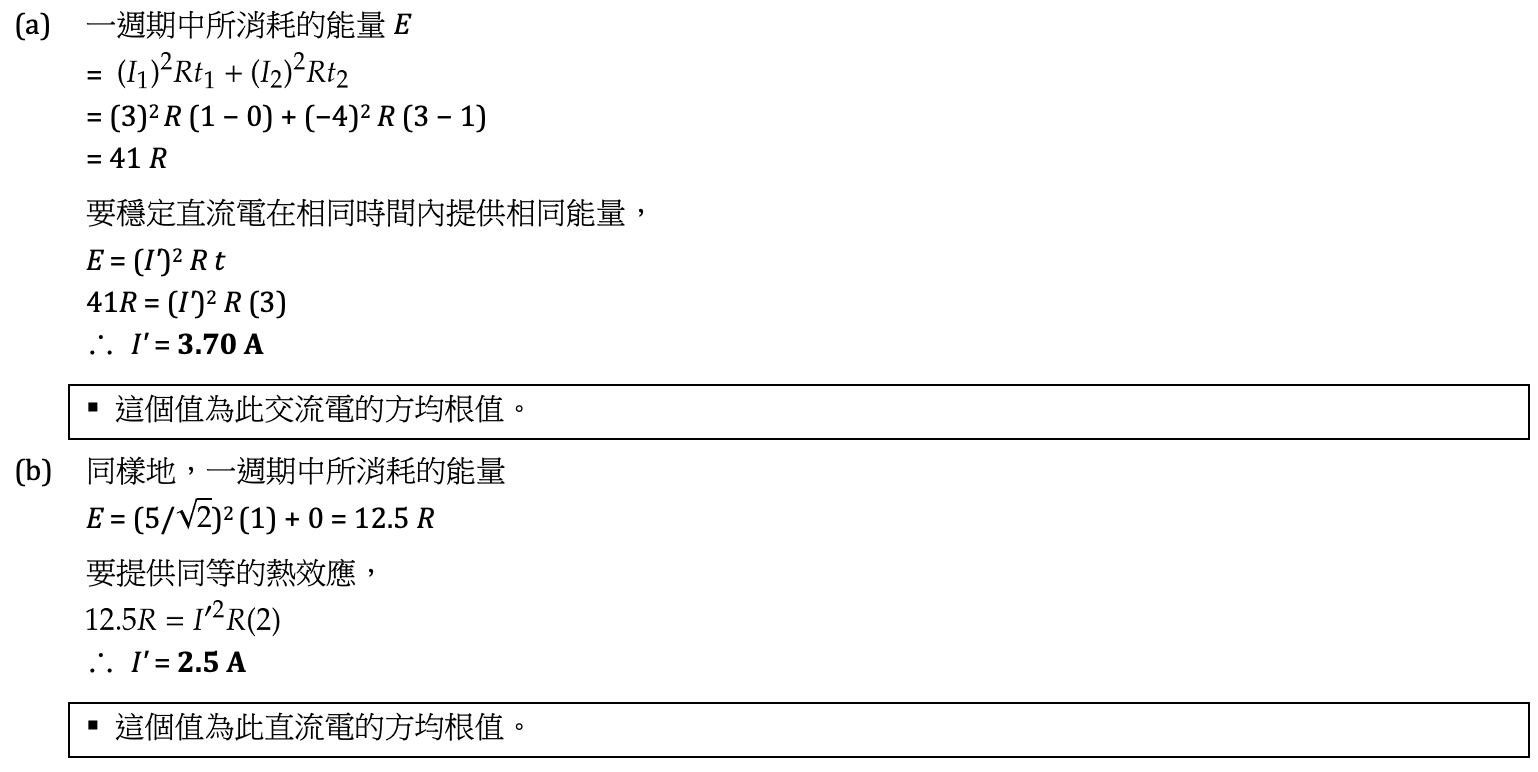
\includegraphics[width=\textwidth]{./img/ch_ACtransformer_lq_2024-06-17-20-35-11.png}\par}
}

\newprob{1718625727}
{
    % Active physics p324 q11
    如圖所示,利用一個 24 V 交流電源,經一個理 恕變壓器操作一個額定值為「120 V,50 W」的 燈泡。
    \par{\par\centering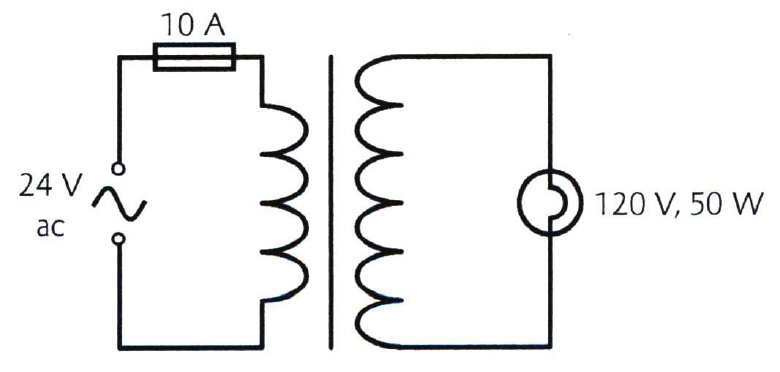
\includegraphics[width=.4\textwidth]{./img/ch_ACtransformer_lq_2024-06-17-20-02-32.png}\par}
    假設燈泡正以額定值運作。
    \begin{parts}
        \part 變壓器的匝數比為多少?\zzh{2}
        \part 逐一以相同燈泡並聯跨接原來的一個。在保 險絲沒有熔斷以前,最多可操作多少個燈 泡?\zzh{2}
    \end{parts}
}{
    % \src{Active physics p324 q11}
    \par{\par\centering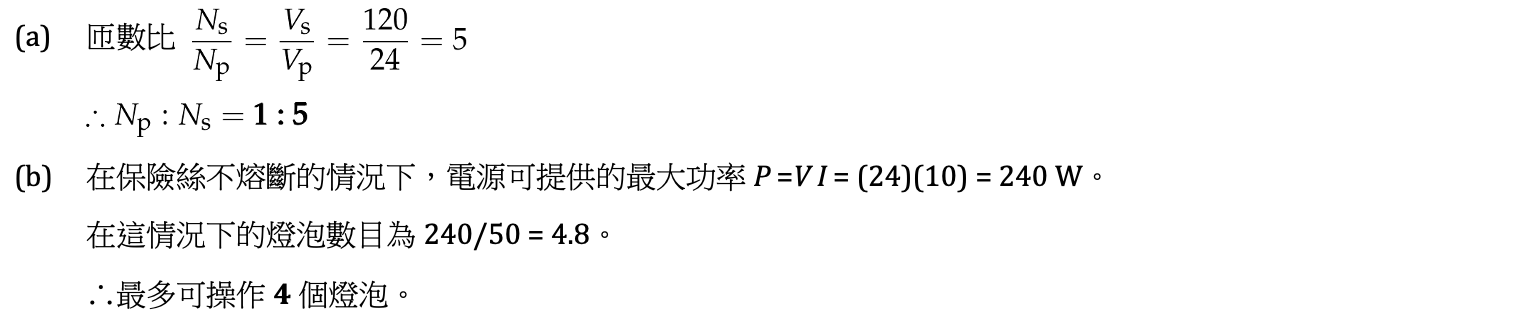
\includegraphics[width=\textwidth]{./img/ch_ACtransformer_lq_2024-06-17-20-37-52.png}\par}
}

\newprob{1718625827}
{
    變壓器採用疊片的鐵心來減少渦電流。以下為三 種疊起薄片的方法。
    \par{\par\centering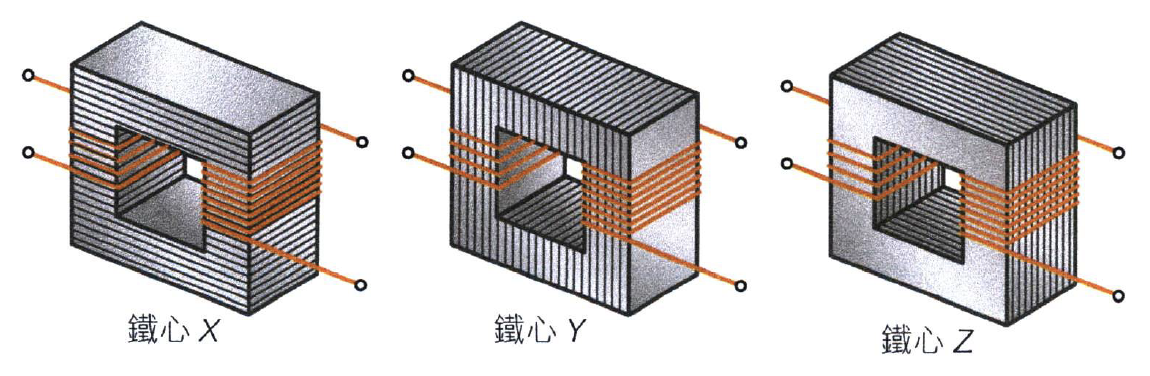
\includegraphics[width=.7\textwidth]{./img/ch_ACtransformer_lq_2024-06-17-20-03-59.png}\par}
    試就變壓器的效率,把鐵心$Z$與另外兩個鐵心$X$和$Y$ 比較。扼要解釋你的答案。\zzh{3}
}{
    % \src{Active physics p324 q13}
    \par{\par\centering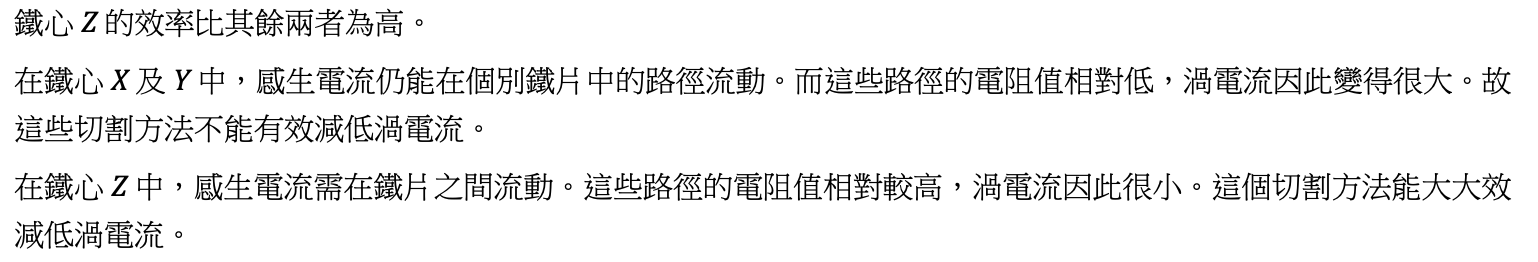
\includegraphics[width=\textwidth]{./img/ch_ACtransformer_lq_2024-06-17-20-38-16.png}\par}
}

\newprob{1718625876}
{
    一個變壓器的原線圈連接至一個24 V交流電 源,副線圈則如圖示般抽頭。兩個燈泡連接至這 個變壓器,並分別以額定值「6 V,50 W」和 「14 V,100 W」運作。
    \par{\par\centering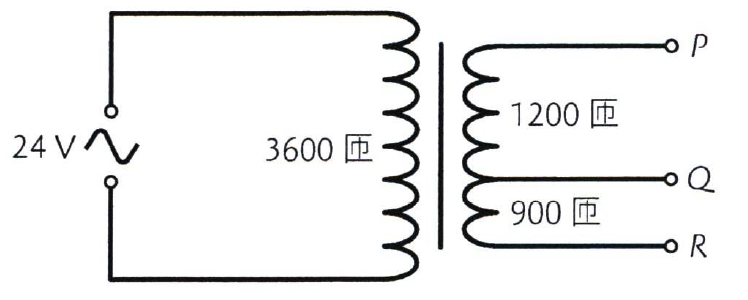
\includegraphics[width=.45\textwidth]{./img/ch_ACtransformer_lq_2024-06-17-20-05-52.png}\par}
    \begin{parts}
        \part 兩個燈泡應如何連接至副線圈上?
        \part 已知變壓器的效率為70\%,求原電流。
    \end{parts}
}{
    % \src{Active physics p324 q16}
    \par{\par\centering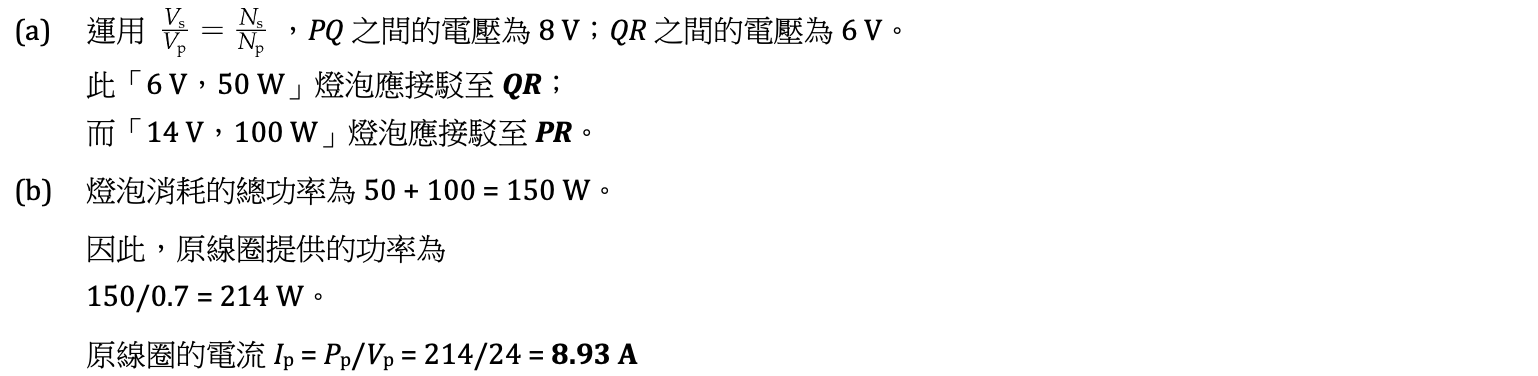
\includegraphics[width=\textwidth]{./img/ch_ACtransformer_lq_2024-06-17-20-38-35.png}\par}
}

\newprob{1718626391}
{
    在發電廠,電力生產時的電壓為22 kV,若以這 電壓直接輸電,功率損耗便為$50\%$。若要把損耗 降至$1\%$,輸電所需的電壓為多少?\zzh{2}
}{
    % \src{Active physics p330 q6}
    \par{\par\centering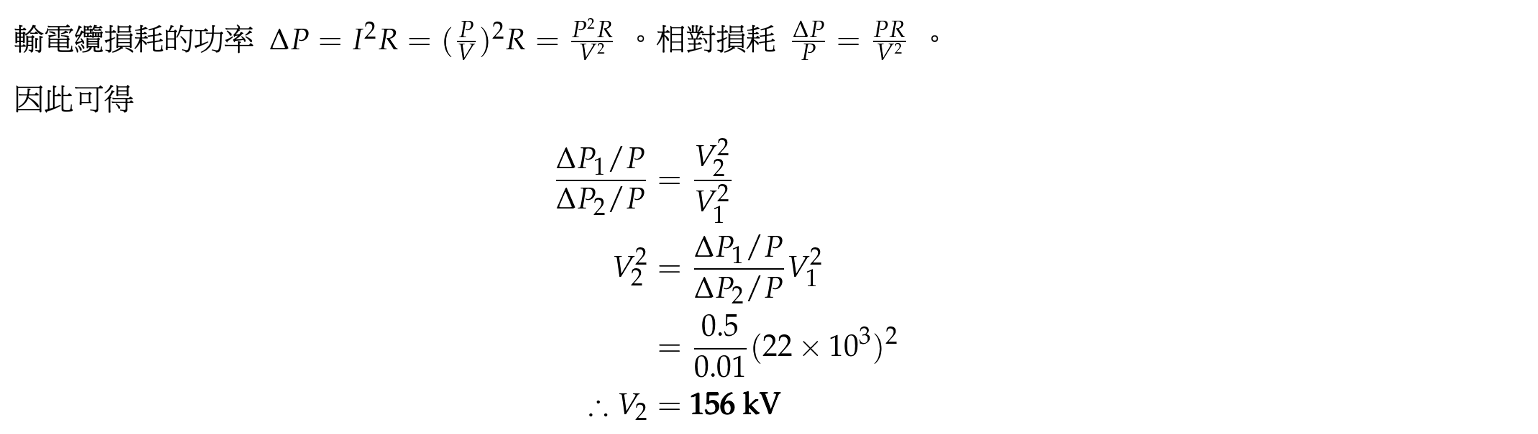
\includegraphics[width=\textwidth]{./img/ch_ACtransformer_lq_2024-06-17-20-39-28.png}\par}
}

\newprob{1718626443}
{
    % Active physics p337 q17
    下圖顯示一個簡單的輸電系統。發電廠所生產的 電力通過輸電纜傳送前,會先以變壓器$X$提升電 壓。
    \par{\par\centering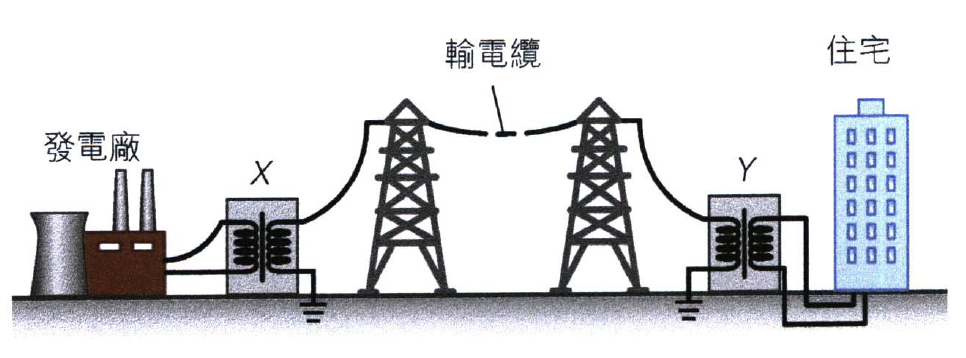
\includegraphics[width=.5\textwidth]{./img/ch_ACtransformer_lq_2024-06-17-20-14-49.png}\par}
    其後,變壓器$Y$會把電壓從50 kV降低至 220 V,再分配至一般住宅用戶。假設某住戶獲得 的總電流為50 A,兩個變壓器的效率為$95\%$。
    \begin{parts}
        \part 發電廠輸出的是直流電,還是交流電?為甚 麼? \zzh{2}
        \part 為甚麼電力以高電壓輸送?\zzh{1}
        \part 輸電纜的總電阻為 \qty{150}{\ohm}。試找出
        \begin{subparts}
            \subpart 輸電纜中的電勢差,以及\zzh{3}
            \subpart 輸電纜中的功率損耗。\zzh{2}
        \end{subparts}
        \part 試估計有用輸出功率的百分比。(有用功率即 住宅用戶的耗電功率) \zzh{2}
    \end{parts}
    \dlines{1}\clearpage
}{
    % \src{Active physics p337 q17}
    \par{\par\centering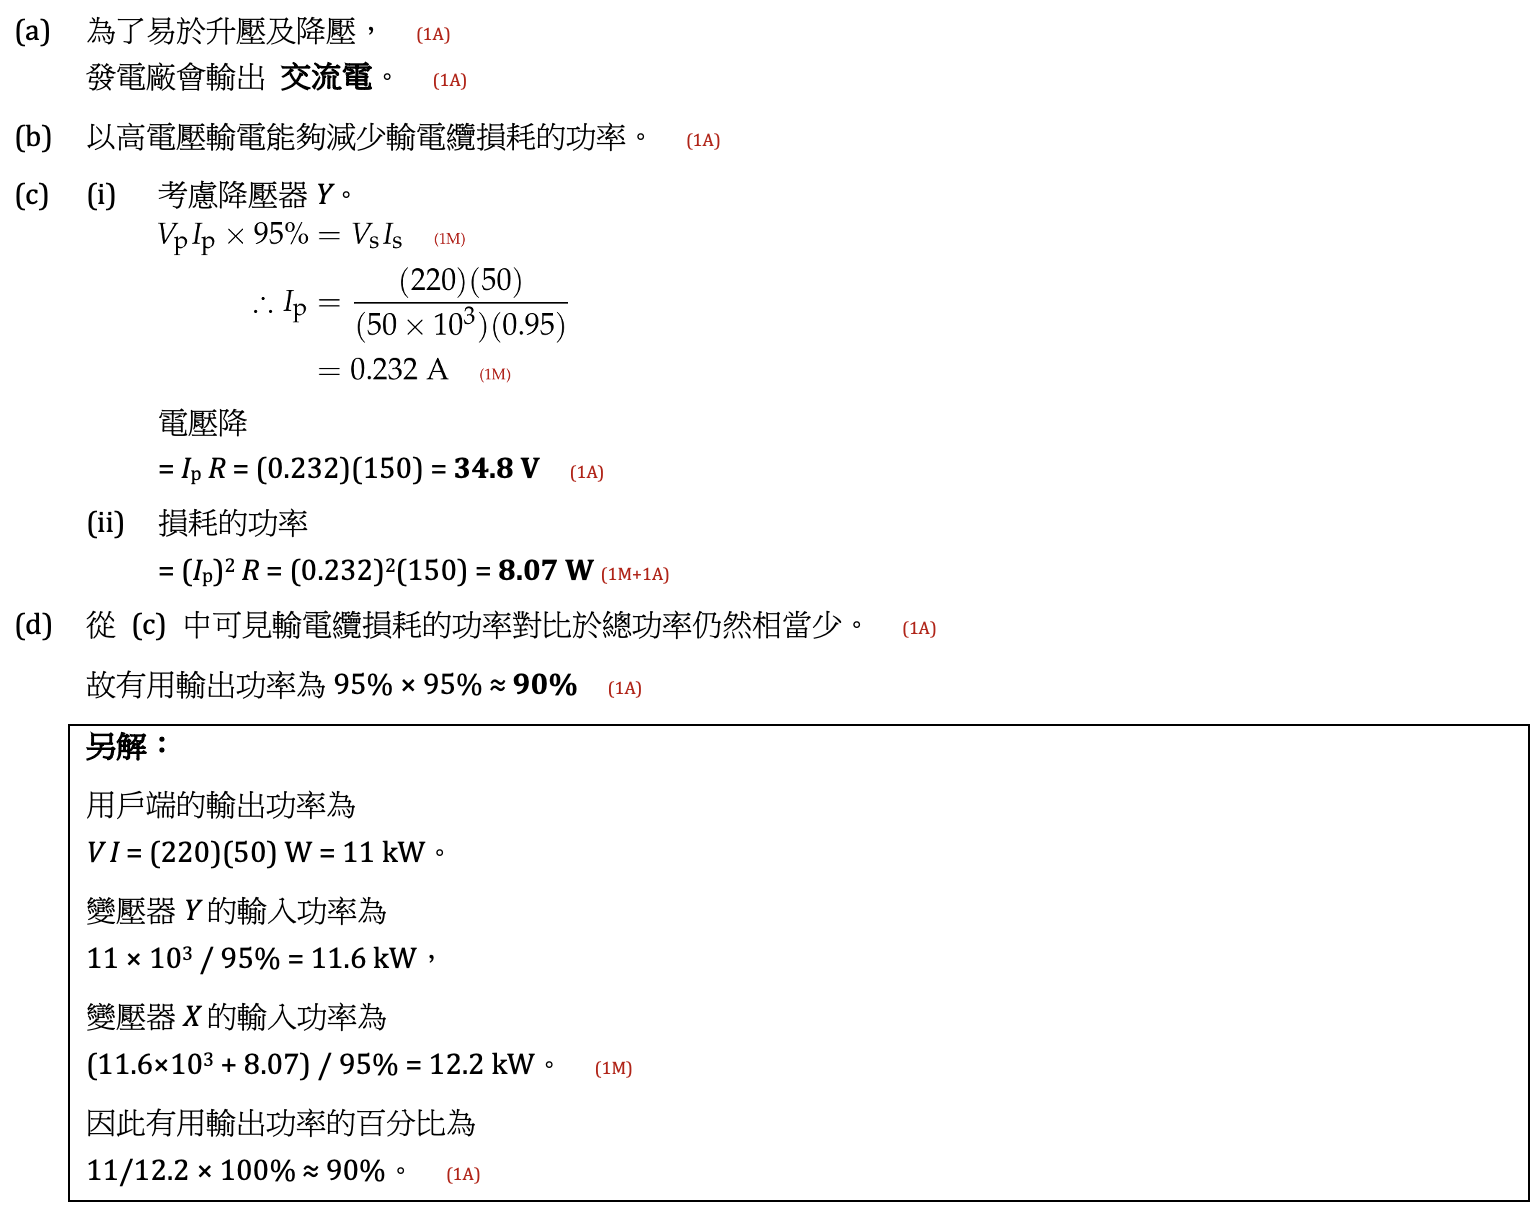
\includegraphics[width=\textwidth]{./img/ch_ACtransformer_lq_2024-06-17-20-40-01.png}\par}
}
